% !TEX TS-program = pdflatexmk
\documentclass[12pt, letterpaper, titlepage]{article}

\makeatletter
\g@addto@macro\@floatboxreset\centering
\makeatother

\usepackage{amsmath}
\usepackage{booktabs}
\usepackage{amsthm}
\usepackage{graphicx}
\usepackage[margin=1in]{geometry}
\usepackage{hyperref}
\hypersetup{colorlinks = true, linkcolor = blue, citecolor=blue, urlcolor = blue}
\usepackage{natbib}
\usepackage{enumitem}
\usepackage{float}
\usepackage{tikz}
\usepackage{setspace}

\usepackage[pagewise]{lineno}
%\linenumbers*[1]
% %% patches to make lineno work better with amsmath
\newcommand*\patchAmsMathEnvironmentForLineno[1]{%
 \expandafter\let\csname old#1\expandafter\endcsname\csname #1\endcsname
 \expandafter\let\csname oldend#1\expandafter\endcsname\csname end#1\endcsname
 \renewenvironment{#1}%
 {\linenomath\csname old#1\endcsname}%
 {\csname oldend#1\endcsname\endlinenomath}}%
\newcommand*\patchBothAmsMathEnvironmentsForLineno[1]{%
 \patchAmsMathEnvironmentForLineno{#1}%
 \patchAmsMathEnvironmentForLineno{#1*}}%

\AtBeginDocument{%
 \patchBothAmsMathEnvironmentsForLineno{equation}%
 \patchBothAmsMathEnvironmentsForLineno{align}%
 \patchBothAmsMathEnvironmentsForLineno{flalign}%
 \patchBothAmsMathEnvironmentsForLineno{alignat}%
 \patchBothAmsMathEnvironmentsForLineno{gather}%
 \patchBothAmsMathEnvironmentsForLineno{multline}%
}

% control floats
\renewcommand\floatpagefraction{.9}
\renewcommand\topfraction{.9}
\renewcommand\bottomfraction{.9}
\renewcommand\textfraction{.1}
\setcounter{totalnumber}{50}
\setcounter{topnumber}{50}
\setcounter{bottomnumber}{50}

\newcommand{\jy}[1]{\textcolor{blue}{JY: #1}}
\newcommand{\eds}[1]{\textcolor{red}{EDS: (#1)}}

%% meta data

\title{Sentiment Analysis of Twitter in Relation to Fossil Fuel Stock Prices}
\author{Pranav Tavildar\\
  University of Connecticut
}

\begin{document}
\maketitle
\doublespace

\begin{abstract}
As a publicly traded company, the Chevron Corporation has the 11th highest market capitalization in the world with 361.57 billion dollars in traded stocks. There exist many social factors that contribute to this stock value but in this paper we seek to determine whether it is possible to see if any of these factors are reflected in public sentiment which can be observed in twitter.  This is done by using a BERT transformer architecture to assign a sentiment score for each tweet and afterwords, we try to determine if there is a correlation between stock price and daily sentiment using an ARMA GARCH Model.

\bigskip
\noindent{\sc Keywords}:
BERT;
chevron;
twitter;
nlp;
sentiment analysis.

\end{abstract}

%%%%%%%%%%%%%%%%%%%%%%%%%%%%%%%%%%%%%%%%%%%%%%%
\section{Introduction}
\label{sec: intro}
%\paragraph{Overview of topic}
\paragraph{}
	The Chevron Corporation is an America-based energy company thats has operations in over 180 countries where it has vertically integrated all operations in its supply chain such as exploration, production, refinement, chemical manufacturing, transportation, sales, marketing, and power generation. A lot of revenue comes from these streams but they also receive funding from government subsidies and stock revenue. As of when this paper was written, the Chevron Corporation has the 11th highest market capitalization with 361.57 billion dollars in traded stocks.
	\paragraph{}
	As a publicly traded company, Chevron's stock price is determined by supply and demand in the market. Generally, this is influenced by factors such as market dynamics, economic conditions and changes to economic policy. Through this paper, we seek to determine whether this can be predicted or determined through observing public speculation on Twitter, the "virtual public square." Being able to determine whether there exists a correlation between public sentiment and the stock price might prove as a valuable indicator for many groups such as investors, activists, and companies officials to determine how much of a correlation a change in public opinion has to the stock value.  	
%\paragraph{Review of the Literature}
\paragraph{}
	To quantify public opinion, this paper uses a machine learning technique known as sentiment analysis \citep{medhat2014sentiment} which uses natural language processing to determine whether the sentiment towards any subject is positive or negative and assigns it a score.
\paragraph{}
	 Some papers in the literature use this technique in relation to analyzing activity in the stock market. Koosha Golmohammadi and Osmar R. Zaiane for instance use sentiment analysis with Twitter data to improve their Contextual Anomaly Detection(CAD) model in order to detect Market Manipulation in the United States and Canada \citep{golmohammadi2017sentiment}. Furthermore, Lu-Tao Zhao and Guan-Rong Zheng web text and applied Sentiment Analysis in order to do Oil Price forecasting \citep{zhao2019forecasting}. This concept has also been applied in order to predict one step ahead of the closing price of the stock market in Thailand using a hybrid model composed of Principle Component Analysis (PCA) for Data Processing (Dimensionality Reduction), Empirical Mode Distribution (EMD) for signal interpretation and data preprocessing, and the Long-Short-Term-Memory(LSTM) model, a specialized type of recurrent neural network for the sentiment analysis. \citep{srijiranon2022hybrid}
\paragraph{}
	While these methods have been tried and proven, as of writing this, the preferred method of analyzing sequence data for most natural language processing is through the use of transformer models. This type of model was first introduced in the paper "Attention is all you need" \citep{vaswani2017attention}. 
\paragraph{}
	This model sought to improve the problems existing with the Recurrent Neural Network(RNN) model which used to be the preferred model for language processing tasks. Transformers have shown a lot of promise, outperforming its competitors in speed and accuracy for natural language processing tasks. Due to its novelty and its promising qualities, many are applying Transformers for various tasks, yet nobody has this used this approach to find out whether it is possible to find out the correlation between Twitter Sentiment and Stock prices of prominent fossil fuel corporations. In this paper, we specifically will focus on the Chevron Corporation (though in future iterations, we might extend this to multiple corporations in this field).
%\paragraph{My Contribution}
\paragraph{}
	In this paper, we will explore using a BERT Transformer model to generate sentiment scores of twitter data from the year 2021 and compare with the 2021 stock prices of the Chevron Corporation (CVX) to determine whether there exists any significant correlation. 
\paragraph{}
	This following is a roadmap for this study: 1) Describing the Data, 2) Explaining the Statistical Methods and the Machine Learning Concepts, 3) Explaining the Results of our Paper, 4) Conducting Discussion of this Study

%%%%%%%%%%%%%%%%%%%%%%%%%%%%%%%%%%%%%%%%%%%%%%%
\label{sec: datadesc}
\section{Data Description}
\paragraph{}
	We use two datasets for this paper: topical twitter tweets from the year 2021 and historical stock data for CVX for the year 2021. 
%%\paragraph{how the economic data was obtained}
\paragraph{}
	Gathering the Historic Stock data was the easiest part of the data collection process. The collection was done through Yahoo Finance's Historical Stock Data tool. The following is a plot of the highs and lows for the year 2021 generated using the matplotlib package for python \citep{Hunter_2007}.

\begin{figure}[!hb]
  \begin{center}
  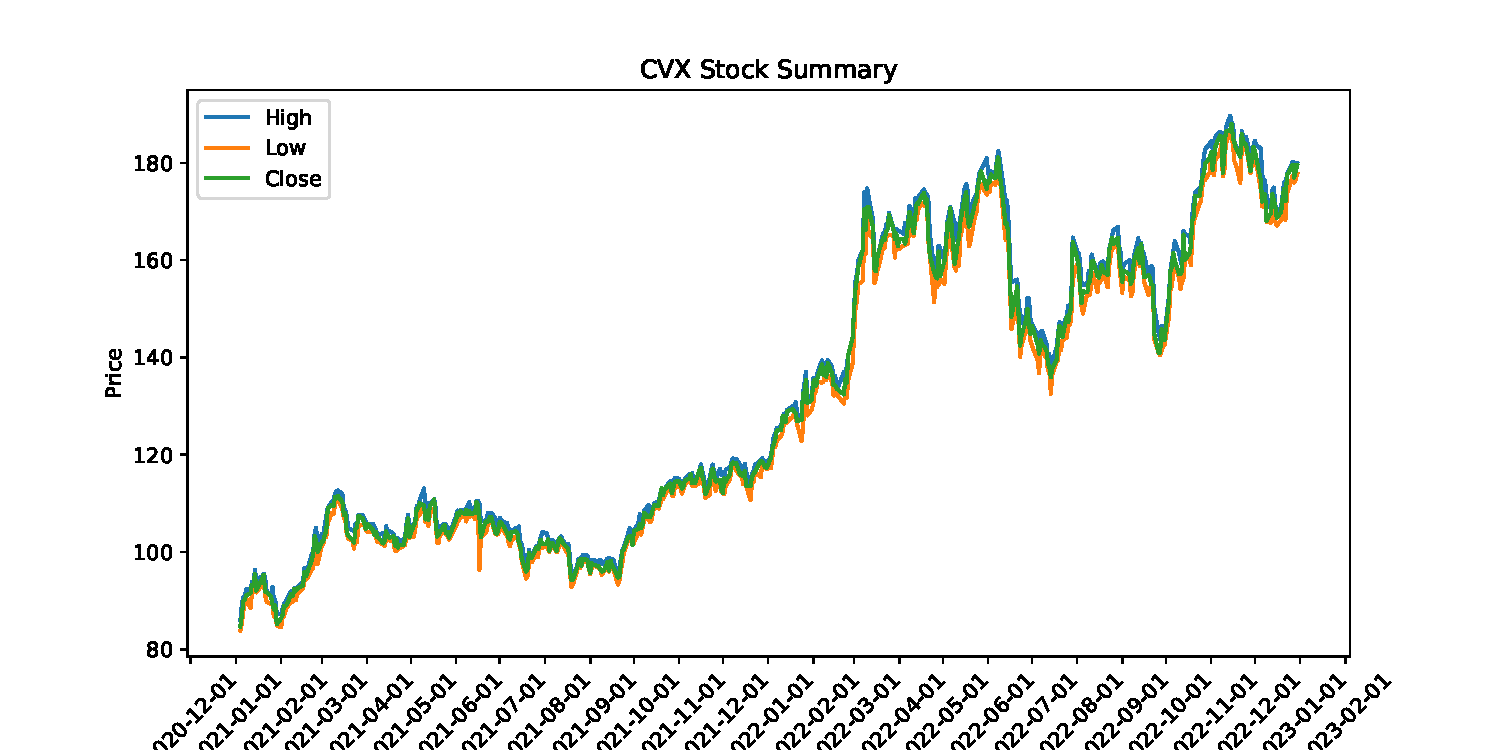
\includegraphics[width=\textwidth]{../figures/fig1.pdf}
  \caption{Here we can see the fluctuations of the highs and lows for the stock price of CVX in 2021 with the highs labeled blue and the lows labeled yellow. In general both values tend to follow each other.}\label{fig:fig1}
  \end{center}
\end{figure}

\paragraph{}
	We also used the data processing library Pandas in order to generate summary statistics as shown below:

\begin{table}[!hb]
  \begin{center}
    \caption{Summary Statistics for the Chevron Stock data}
    \label{tab:table1}
    \begin{tabular}{l|c|r} % <-- Alignments: 1st column left, 2nd middle and 3rd right, with vertical lines in between
      \textbf{Metrics} & \textbf{High} & \textbf{Low}\\
      \hline
      count & 251.000000 & 251.000000\\
      mean & 105.196175 & 103.091753\\
      std & 7.747654 & 7.814207\\
      min & 85.949997 & 83.889999\\
      25\% & 99.900002 & 97.724998\\
      50\% & 105.080002 & 102.970001\\
      75\% & 110.330002 & 107.969998\\
      max & 119.339996 & 118.040001\\
    \end{tabular}
  \end{center}
\end{table}

	
\paragraph{}
	The range of the stock value goes from 83.889 to 119.336 and is representative of the stock prices from January 4th, 2021 to December 30th, 2021. There are 251 days that the stock data was available for in 2021. This is because Chevron is a part of the New York Stock Exchange which is closed all day on Saturdays, Sundays and nine holidays a year. This was something that was taken into consideration when working with twitter data. 

\paragraph{}
	The twitter data was scraped using the python package snscrape \citep{justanotherarchivist_2022}. This is an open source library that allows for the scraping of twitter data without having to use the API. The code used to generate the twitter data can be found in code/datagen.py. In short, the process used to scrape the data was to first create some auxiliary functions for tasks such as determining how many tweets need to be gathered at a given time and create some functions to make it easier to pass in queries in the Twitter Search Scraper object. There are 2 things you can query for and that is by using either some topic keywords or the tweets from a specific user. 
	
\paragraph{}
	For the purpose of this paper, we scraped 5 tweets a day with the topic query "Chevron Oil" from January 1st 2021 to December 31st.  We then saved all the 1825 generated tweets as a csv and merged them with the CVX stock data on the Date axis after matching datatypes. This also omitted tweets which were created when the stock market was closed in order to simplify the analysis. Using this we were able to perform sentiment and calculate correlation.


%%%%%%%%%%%%%%%%%%%%%%%%%%%%%%%%%%%%%%%%%%%%%%%
\label{sec: methods}
\section{Methods}

\subsection{Data Collection}
Twitter data related to the Chevron Corporation was collected using web scraping techniques. Specifically, tweets containing the term "CVX" were extracted from Twitter using the topic selection method provided by the snscrape\citep{justanotherarchivist_2022} Python wrapper. The tweets were collected for a period of 2 years, from January 1, 2021 to December 31, 2022 with 10 tweets being collected each day.

\subsection{Sentiment Analysis}
\paragraph{The Transformer Model}
	As we mentioned earlier, Transformers have shown a lot of promise, outperforming its competitors in speed and accuracy for natural language processing tasks. The BERT model seems to be particularly well suited for tasks of sentiment analysis. Transformers work based on the concept of "attention" which was introduced in "Attention is all you need" \citep{vaswani2017attention} is a deep learning model that was first used for computer vision models. Transformers create differential weights signaling which words in a sentence are the most critical to further process. This allows them to "forget"  irrelevant information which would use other critical resources.
	

\begin{figure}[H]
\tikzset{every picture/.style={line width=0.75pt}} %set default line width to 0.75pt        
\begin{tikzpicture}[x=0.75pt,y=0.75pt,yscale=-1,xscale=1]
%uncomment if require: \path (0,300); %set diagram left start at 0, and has height of 300
%Rounded Rect [id:dp4434986972980839] 
\draw   (100,43.8) .. controls (100,32.76) and (108.95,23.8) .. (120,23.8) -- (261,23.8) .. controls (272.05,23.8) and (281,32.76) .. (281,43.8) -- (281,103.8) .. controls (281,114.85) and (272.05,123.8) .. (261,123.8) -- (120,123.8) .. controls (108.95,123.8) and (100,114.85) .. (100,103.8) -- cycle ;
%Rounded Rect [id:dp8739677930569794] 
\draw   (359,68.2) .. controls (359,52.52) and (371.72,39.8) .. (387.4,39.8) -- (472.6,39.8) .. controls (488.28,39.8) and (501,52.52) .. (501,68.2) -- (501,168.4) .. controls (501,184.09) and (488.28,196.8) .. (472.6,196.8) -- (387.4,196.8) .. controls (371.72,196.8) and (359,184.09) .. (359,168.4) -- cycle ;
%Curve Lines [id:da9359490056283244] 
\draw    (282,73) .. controls (362,56.8) and (275,143.8) .. (359,124.8) ;
%Straight Lines [id:da03881732608220867] 
\draw    (78,72.8) -- (101,73) ;
%Straight Lines [id:da6091063106538472] 
\draw    (500,120.8) -- (523,121) ;
%Straight Lines [id:da19347919375178857] 
\draw    (431,215.8) -- (431,199.8) ;
% Text Node
\draw (161,65) node [anchor=north west][inner sep=0.75pt]   [align=left] {Encoder};
% Text Node
\draw (398,103) node [anchor=north west][inner sep=0.75pt]   [align=left] {Decoder};
% Text Node
\draw (42,63) node [anchor=north west][inner sep=0.75pt]   [align=left] {Input};
% Text Node
\draw (524,112) node [anchor=north west][inner sep=0.75pt]   [align=left] {Output};
% Text Node
\draw (408,219) node [anchor=north west][inner sep=0.75pt]   [align=left] { Output Probabilites};
\end{tikzpicture}
\caption{In this figure we can observe a very simplified version of the Transformer model with its two major components, the encoder and the decoder. The encoder processes a text input through a stack of transformer layers. In some situations, another set of transformer layers, the decoder, can be used to predict a target output. Note that this model might be used for a task such as language translation.\citep{devlin2018bert}}\label{fig:fig2}
\end{figure}

\paragraph{}
We will be utilizing Bidirectional Encoder Representations from Transformers (BERT) for our sentiment analysis. BERT is a transformer model developed by Google that can perform multiple Natural Language Processing tasks such as sentiment analysis, text classification, chatbots, text extraction, machine translation, text summarization, market intelligence, auto-correct, intent classification, urgency detection, and speech recognition.

\paragraph{}
This model was initially trained on Wikipedia and Google’s BooksCorpus which contain 2,500,000,000 words and 800,000,000 words respectively. Training of BERT was completed over a period of 4 days using 64 Tensor Processing Units running in parallel. With this much data, it is able to understand context clues making it a very effective model for the purposes of sentiment analysis.

\paragraph{}
We will be specifically using BERT-base which is a version of BERT with 12 transformation layers, and 768 Hidden Layers.\citep{muller_2022} This is more reasonable for the task we have at hand and we will implement this using the Hugging Face transformers package. For each day, the average sentiment score of all tweets was calculated. Sentiment scores range from -1 to 1, where -1 represents a very negative sentiment and 1 represents a very positive sentiment.

\subsection{ARMA-GARCH Modeling}
The daily returns for Chevron's stock (CVX) were obtained from calculating as the daily logarithmic difference of the closing prices. ARMA-GARCH modeling was then performed to investigate the relationship between the daily returns and the sentiment scores.

First, an ARMA model was selected for the returns using the \texttt{auto.arima} function in the forecast package in R. The \texttt{max.D} and \texttt{max.d} parameters were set to 0 to avoid differencing in the ARMA model.

Next, a GARCH model was fitted to the ARMA residuals using the \texttt{ugarchfit} function in the rugarch package in R. The sGARCH model was used for the variance with an order of (1,1) and the mean was modeled using the ARMA model selected earlier.

To investigate the impact of sentiment on stock returns, an ARIMAX model was fitted to the returns using the \texttt{arimax} function in the TSA package in R. The daily sentiment scores were included as an exogenous variable. An ARIMAX model was also fitted to the sentiment scores using the \texttt{auto.arima} function in the forecast package in R.

Finally, a GARCHX model was fitted to the returns with sentiment scores using the \texttt{garchx} function in the garchx package in R. The order was set to (1,1), and the initial values for the GARCH coefficients were taken from the ARMA-GARCH model.

For further analysis, a weighted sentiment score was calculated by assigning a weight to each sentiment score based on the number of tweets collected for that day. The weighted sentiment score was then used as an exogenous variable in the ARIMAX and GARCHX models, and the results were compared to those obtained using the unweighted sentiment score.

%%%%%%%%%%%%%%%%%%%%%%%%%%%%%%%%%%%%%%%%%%%%%%%
\label{sec: results}
\section{Results}
\paragraph{}
The sentiment analysis took approximately 12 minutes to run and the data generated created 3 new columns in the working dataframe: sentiment, label, and score. Score is a numeric value from the range [0,1] where the higher the score the more confident the sentiment analyzed is correct. This variable is one of interest to us since we want to use it to measure correlation with highs of the stock market The summary statistics listed the following:

\begin{table}[!hb]
  \begin{center}
    \caption{Summary Statistics for the Sentiment Analysis of Tweets}
    \label{tab:table2}
    \begin{tabular}{l|c|r} % <-- Alignments: 1st column left, 2nd middle and 3rd right, with vertical lines in between
      \textbf{Metrics} & \textbf{High} \\
      \hline
      count & 1160 \\
      mean & 0.960652 \\
      std & 0.086946 \\
      min & 0.500485 \\
      25\% & 0.9740872 \\
      50\% & 0.992183 \\
      75\% & 0.997086 \\
      max & 0.999799 \\
    \end{tabular}
  \end{center}
\end{table}

\paragraph{}
To calculate correlation, we must make sure that the fundamental assumptions are satisfied. The data is continuous and monotonic so we can proceed with Kendall's correlation. We used pandas to calculate Kendall's correlation. The following is a heat map of the correlation plotted using the seaborn package for python \citep{Waskom2021}.

\begin{figure}[H]
  \begin{center}
  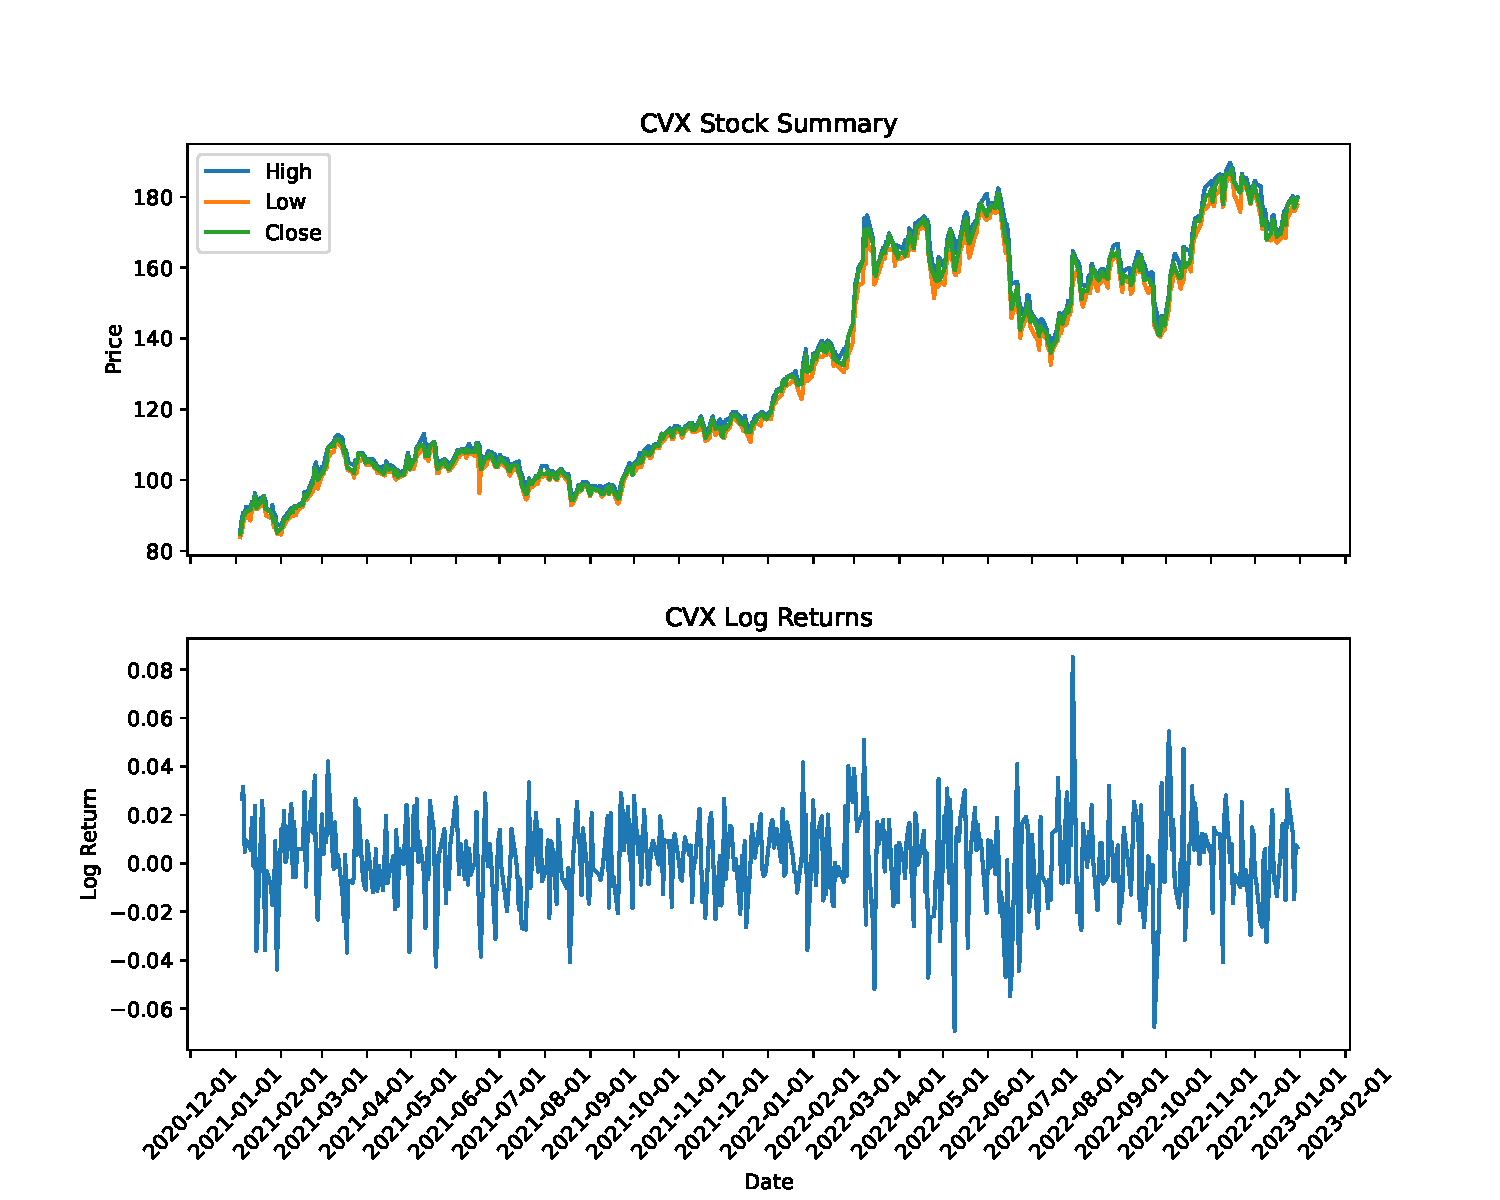
\includegraphics[width=\textwidth]{../figures/fig2.pdf}
  \caption{Here we can observe the correlation between sentiment score and stock high price. The value is -0.009447. }\label{fig:fig2}
  \end{center}
\end{figure}

Given that the correlation it is negative, this indicates that there is a very minor inverse relationship between score and stock price. But given how low it is, this result is practically negligible and it appears that there is almost 0 correlation between the variables we are measuring. This indicates a lot of revision being needed for the data and methods of analysis in this paper.
%%%%%%%%%%%%%%%%%%%%%%%%%%%%%%%%%%%%%%%%%%%%%%%
\label{sec: discussion}
\section{Discussion}
\paragraph{}
	As mentioned before, this paper is the first one to take the approach of using Transformers to determine whether it is possible to find out the correlation between Twitter Sentiment and Stock prices of prominent fossil fuel corporations. In summary, this paper accomplished this task through the following:
\begin{itemize}
    \item Introducing some background behind the Chevron Corporation and Sentiment Analysis as a Practice.
    \item Describing the data and the methods by which the data was obtained.
    \item Describing the methods behind the sentiment analysis and correlation derivation
    \item Describing the results
    Through code and analysis, we were eventually did get a correlation coefficient score of -0.009447 which is very low based on what was expected indicating that there is very little correlation between twitter sentiment and stock price.

\end{itemize}
\paragraph{}
	In its current state, this study is intended to work as a proof of concept to determine whether it is possible to create a data processing pipeline which could be used to assign sentiment scores and connect it to stock time series data so the results determined through this preliminary paper should not be taken as a final answer to the research question that were posed. This study had many limitations which can be addressed to get a more accurate answer. 

	For instance the transformer pipeline model that was used handled cleaning and preprocessing automatically, this might have lead to improper tokenization which allowed for incorrect sentiment analysis. The 18th tweet in merged.csv reads 
	
	"Richmond Mayor Tom Butt was publicly optimistic about a Chevron oil refinery spill. In private he took on a much different tone." 
	
	This was labelled as positive by BERT but in actuality this is a negative tweet.
\paragraph{}
	To avoid instances like this we could also use more terms for the tweet querying such as a specific event such as an oil spill or possibly the stock indicator itself. 

\paragraph{}
The major things to address as next steps are improving the data quality, quantity and analysis. I will also explore using the twitter API to gather tweets instead of using snscrape since the API is the prefered method of gathering tweets in professional contexts and this opens data gathering up to many more possibilities with new methods and feature information that could be gathered using the API query feature.  Having more tweets per day is also beneficial in improving the quality of analysis. 

\paragraph{}
Furthermore, using different data and methods would allow us to possibly create a model that can forecast stock pricing if the correlation is strong enough. This would be done in a manner similarly to \citep{zhao2019forecasting}. 

This project will require much more development and expansion before a conclusion  can be determined but analyzing the effect of public sentiment on stock prices of fossil fuel companies can provide valuable insight into how public opinion can be used to augment or reduce the effects of climate change.
\bigskip
\bigskip
\bigskip
\bigskip
\bigskip
\bigskip
\bigskip
\bigskip
\bigskip
\bigskip
\bigskip
\bigskip
\bigskip
\bigskip
\bigskip
\bigskip
\bigskip
\bigskip
\bigskip
\bigskip
\bigskip
\bigskip
\bigskip
\bigskip
\bibliographystyle{chicago}
\bibliography{references}

\end{document}